\documentclass[10pt,a4paper,twoside,twocolumn]{article}
%% Lots of packages !
\usepackage{etex}

%% Francisation
\usepackage[english]{babel}
\usepackage[T1]{fontenc}
\usepackage[utf8]{inputenc}
%\usepackage{textcomp}

%% Réglages généraux
\usepackage[left=1.5cm,right=1.5cm,top=2cm,bottom=2cm]{geometry}
\usepackage{fancyhdr}
\usepackage{setspace}
\usepackage{lscape}
%\usepackage{multicol}
\usepackage{makeidx}
\usepackage[clearempty]{titlesec}
\usepackage{cite}

%% Packages pour le texte
\usepackage{pifont}
\usepackage{eurosym}
\usepackage{soul}
\usepackage[normalem]{ulem}
\usepackage{fancybox}
\usepackage{boxedminipage}
\usepackage{enumerate}
\usepackage{verbatim}
\usepackage{moreverb}
\usepackage{listings}
\usepackage[table]{xcolor}

%% Packages pour les tableaux
\usepackage{array}
\usepackage{multirow}
\usepackage{tabularx}
\usepackage{longtable}

%% Packages pour les dessins
\usepackage{graphicx}
\usepackage{wrapfig}
%\usepackage{picins}
\usepackage{picinpar}
\usepackage{epic}
\usepackage{eepic}
\usepackage{tikz}
\usepackage{afterpage}
\usepackage{rotating}
\usepackage{float}
\usepackage{caption}

%% Packages pour les maths
\usepackage{amsmath}
\usepackage{amssymb}
\usepackage{dsfont}
\usepackage{mathrsfs}
\usepackage{bussproofs}
\usepackage[thmmarks,amsmath]{ntheorem}

%% Création de nouvelles commandes
%\usepackage{calc}
\usepackage{ifthen}
\usepackage{xspace}



\usepackage{url}
\usepackage{hyperref}
\usepackage{todonotes}
\usepackage{subcaption}
\usepackage[french,ruled,vlined,linesnumbered,algosection,dotocloa]{algorithm2e}
\usepackage{MnSymbol}

\usepackage{chngcntr}

\usepackage{standalone}
\usepackage{import}

\usepackage[affil-it]{authblk}


\usepackage{lipsum}












\numberwithin{equation}{subsection}


\newcommand*{\rootPath}{../}
\standalonetrue

\begin{document}
\section{Memory corruption study}

Memory corruption related error can happen in different ways. Cosmic rays and
radiation have, for a long time, been suspected of creating random data
\todo{ref}. More rescently we realised that thoses error can also happen because
of hardware issues\todo{ref}.

Beyound the question of those corruptions causes, we are here focussing on the
impact such event have on our pipeline.

\subsection{Error classification}

Depending on a large number of factor, memory corruption can have very different
concequences. Such factor include many things from hardware components (ECC
memory one of the most well know mecanism against memory correption) to software
certification and computation redondancy.

As for the consequences, they can be divided into two different categories :
\begin{description}
	\item[Hard errors:] Memory corruption affect the system of the program flow
		will most likely cause dramatic errors such as the program stopping
		abruptly or the whole system failling. In such cases we do not get any
		results back, redering irrelevant the question of the result's validity.
		Some memory corruptions affecting critical data such as table indices also
		falls into this category.

	\item[Silent errors:] Memory corruption in some application's data may not
		cause any crash of the application while affecting the results if not
		corrected by the hardware. This is particularly the case of large array's
		contents like particles positions in our pipeline.
\end{description}

In this section we will try to caracterise silent errors' impact on our
pipeline's results.

\subsection{Corruption injection}

Simulating random memory corruption can be done by voluntarly modifying our
applications data by randomly flipping bits. While this isn't hard to do,
studying silent errors means we have to enshure that those random bit flips will
not cause hard errors.

Differents software quality implies different level of tolerence. For exemple
some code can handle particles positions being outside of our considered domain
while other might crash\todo{harderror ratio for tess ?}. Form here on we will
mostly focus on our AKDE implementation as it very resistant to such errors and
therefore more suitable to create and analyse silent errors.

In our model, simulating memory corruption is achieved by randomly modifying our
input data set. In real application this dataset would be provided by another
program and would have therefor been send through the network of saved on disk,
increasing the probability of memory corruption. This injection model will be
controlled by two parameters, on the one hand the number of bit flips and one
the second hand the weight of the potentially affected bits.

While the first parameter is used to simulate different degre of corruption, the
second one is used to study the impact of differents bit flip position. The
construction of IEEE floating point arithmetics\cite{Kahan1996} (IEEE 754) is
such different bit modification produce different arithmetic modification.

Studies have shown that in some HPC pipelines, some bits' position are critical,
the modification of those bits resulting in hard errors while some other bits' 
modifications are un noticeable as the resulting modification are bellow the
accuracy of floating computation\todo{ref - Leonardo's tech report}.

\subsubsection{Single error injection}

As a first step in our analysis of memory corruption's impact on density
estimator we will study the impact of single bitflip positions.

We are therefore going to modify, for various samplings of our density function,
the value of one randomly selected floating value by flipping it's $n$-th bit.
For single precision floating values this $n$ value varies between $0$ and $31$
as simple precision floating value are $32$ bits long. Once this mofication has
been done, the corrupted sampling is processed by the pipeline and compared to
uncorrupted results.

This single bit flip injection experiment gives expected yet interresting
results.

Injecting a single bit flip moves on particle by modifiying one of its floating
coordinates. While some bit's position only have a small impact, other can have
an impact on the pipeline. Modification of the exponent bits can make the
affected particule exit the donsidered domain, which some code cannot handle.
As a consequensed, some bit flips cause Tess-Dense to crash. Other code, like
our AKDE implementation can handle particle exiting the domain and, for such
corruption in fact produce silent errors.

The first conclusion that some specific memory corruption produce hard errors
due to bad coding practices. Those same memory corruption can in fact be
detected inside the process by checking that the data verify some specific
criterion.

Once the corrupted sampling processed using AKDE, the resulting density could
not be distinguish for expected results ass they where whitin the range of
expected results. This was to be expected has a single memory corruption could
be seen as a verry slight modification of one of many particles in the
intrinsically random sampling and therefore be statically indiscernible.

\subsubsection{Multiple error injection}

As the first approch showed us that single errors are indiscernible, we will now
study the impact of the memory corruption rate on result's quality. For that we
will inject large number of error, randomly distributed throughout out input
data. Our input data are sampling containing :
\begin{table}[!h]
	\centering
	\begin{tabular}{rlcrl}
		$2\times10^5$	& particles	&=	& $6\times10^5$			& floats	\\
									&						&=	& $1,92\times10^7$	& bits
	\end{tabular}
\end{table}
We are here going to inject various number of bit flips (up to $10^6$
independant bit flips) and then evaluate the difference to the expected range.

Figure~\ref{fig:synthetic:corrupted:fields} shows the density field computed by AKDE after
injection of random bit flips.

\begin{figure*}[p]
	\centering
	\includegraphics[width=0.9\textwidth]
		{\rootPath Figures/synthetic/randomized-multiplot.pdf}
	\caption{AKDE density fields after error injection}
	\label{fig:synthetic:corrupted:fields}
\end{figure*}

Beyound the small noise on the sides, made visible by the density log scale, an
cross is visible at the center of the domain. This cross is caused by bit flips
in exponent part of floating point values, making them converge toward $0$. We
therefore have a high density around plane $\mathcal P_{x=0}$,
$\mathcal  P_{y=0}$ and $\mathcal P_{z=0}$.

Figure~\ref{fig:synthetic:corrupted:spectrum} shows the power spectrum of those density
fields.

\begin{figure*}[p]
	\centering
	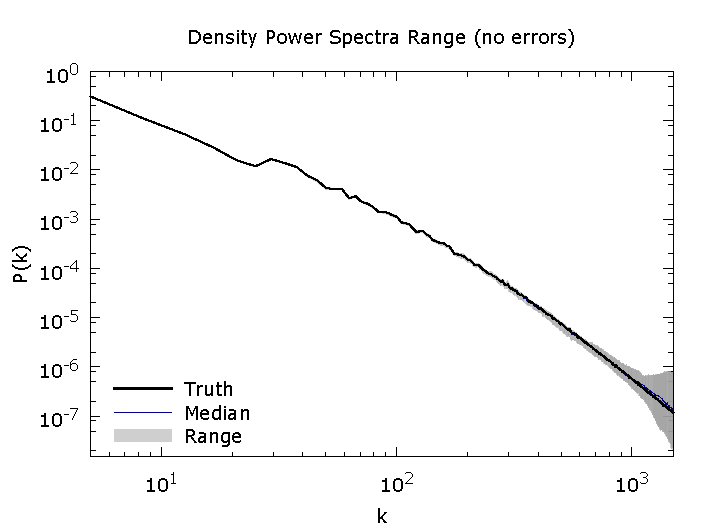
\includegraphics[width=0.32\textwidth]
		{\rootPath Figures/synthetic/psd-errors/cnfw_particles_2e5_akde_err0_clamped.pdf}
	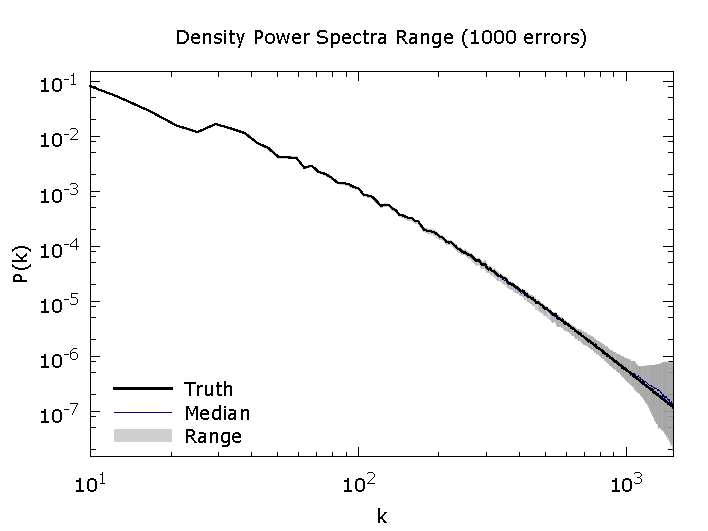
\includegraphics[width=0.32\textwidth]
		{\rootPath Figures/synthetic/psd-errors/cnfw_particles_2e5_akde_err1000_clamped.pdf}
	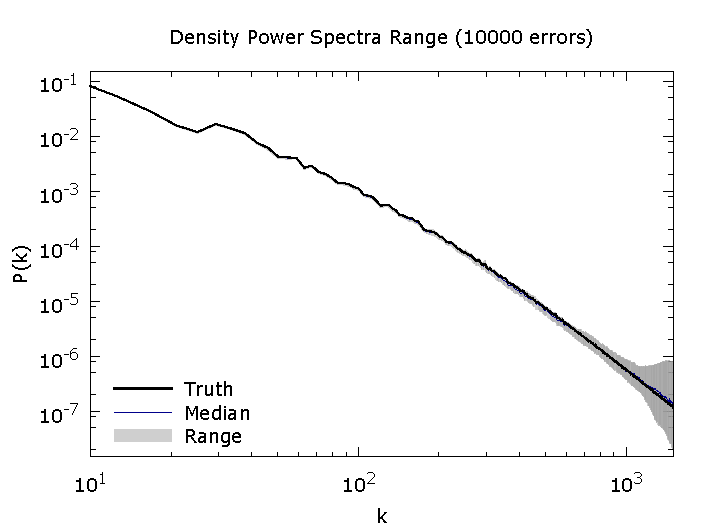
\includegraphics[width=0.32\textwidth]
		{\rootPath Figures/synthetic/psd-errors/cnfw_particles_2e5_akde_err10000_clamped.pdf}
	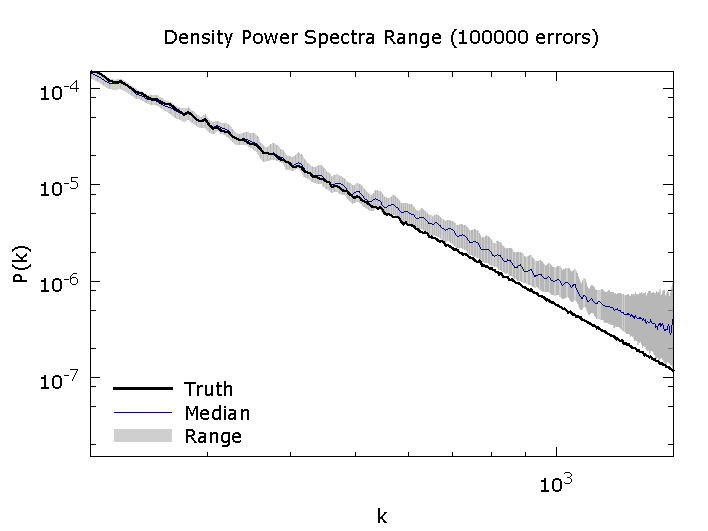
\includegraphics[width=0.32\textwidth]
		{\rootPath Figures/synthetic/psd-errors/cnfw_particles_2e5_akde_err100000_clamped.pdf}
	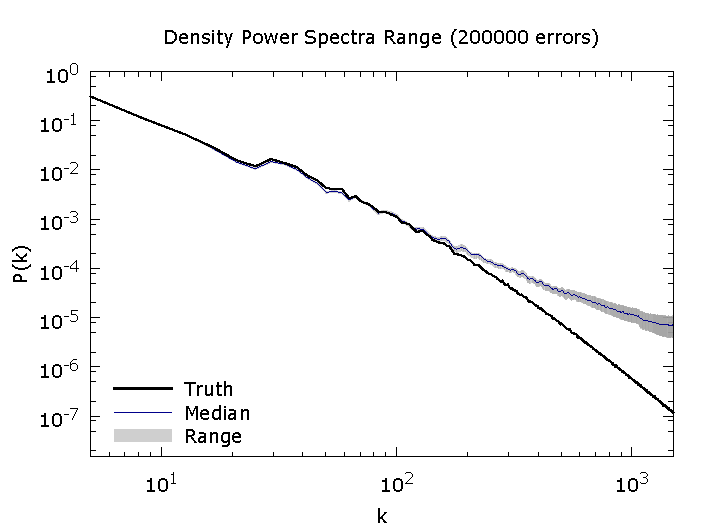
\includegraphics[width=0.32\textwidth]
		{\rootPath Figures/synthetic/psd-errors/cnfw_particles_2e5_akde_err200000_clamped.pdf}
	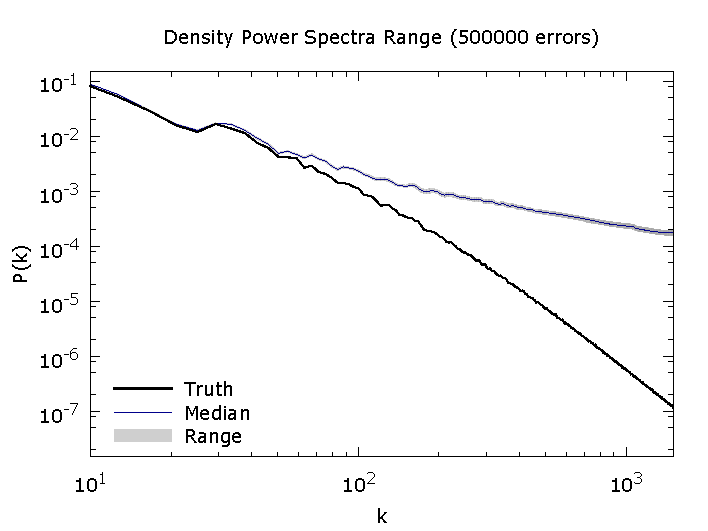
\includegraphics[width=0.32\textwidth]
		{\rootPath Figures/synthetic/psd-errors/cnfw_particles_2e5_akde_err500000_clamped.pdf}
	\caption{Bitflip influence on AKDE power spectrum range}
	\label{fig:synthetic:corrupted:spectrum}
\end{figure*}

Those results both show a discrepancy between corrupted pipeline and expected 
results for error numbers between $10^4$ and $10^5$.






\begin{figure*}[p]
	\centering
	\includegraphics[width=0.9\textwidth]
		{\rootPath Figures/hacc/randomized-multiplot.pdf}
	\caption{AKDE density fields after error injection}
	\label{fig:hacc:corrupted:fields}
\end{figure*}


\begin{figure*}[p]
	\centering
	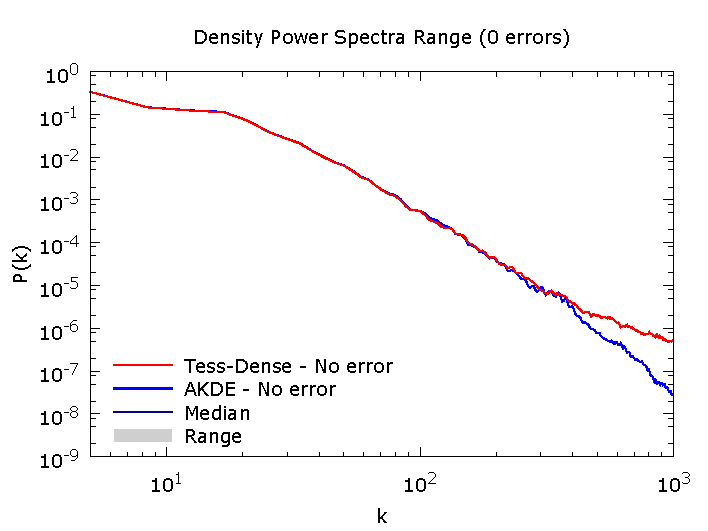
\includegraphics[width=0.32\textwidth]
		{\rootPath Figures/hacc/psd-errors/trace_255_akde_err0.pdf}
	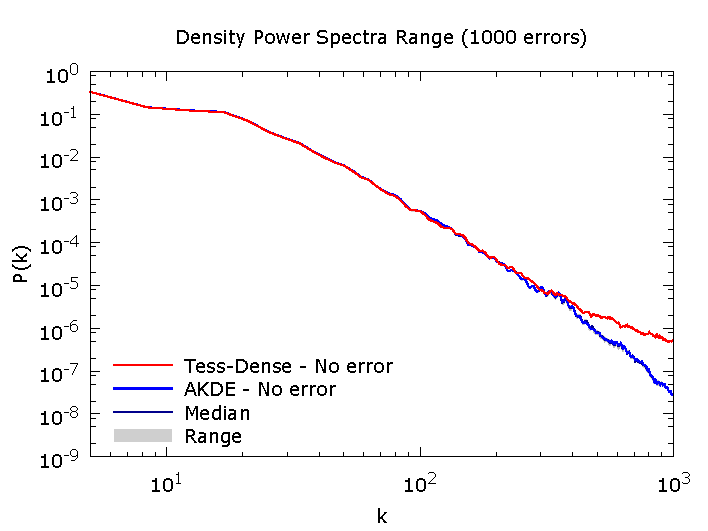
\includegraphics[width=0.32\textwidth]
		{\rootPath Figures/hacc/psd-errors/trace_255_akde_err1000.pdf}
	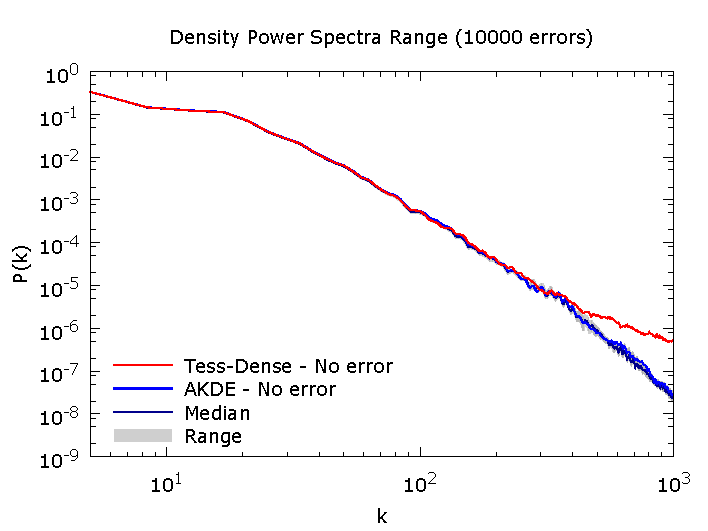
\includegraphics[width=0.32\textwidth]
		{\rootPath Figures/hacc/psd-errors/trace_255_akde_err10000.pdf}
	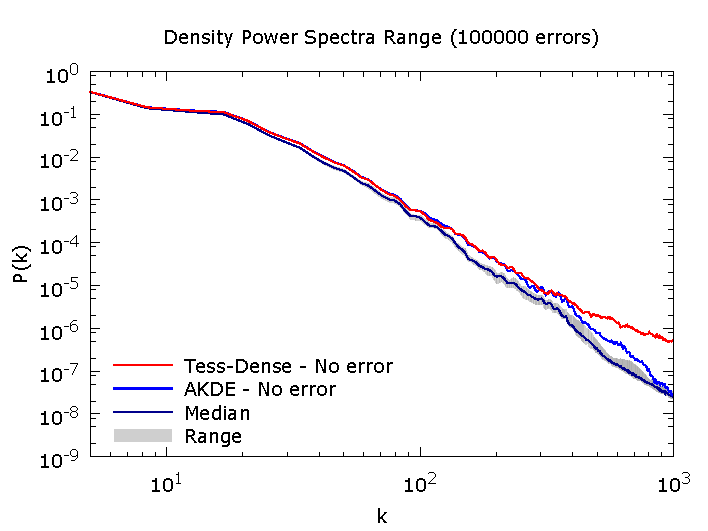
\includegraphics[width=0.32\textwidth]
		{\rootPath Figures/hacc/psd-errors/trace_255_akde_err100000.pdf}
	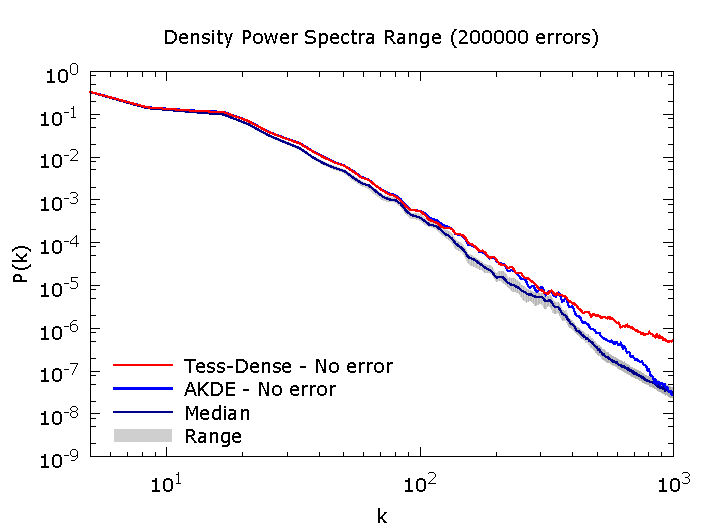
\includegraphics[width=0.32\textwidth]
		{\rootPath Figures/hacc/psd-errors/trace_255_akde_err200000.pdf}
	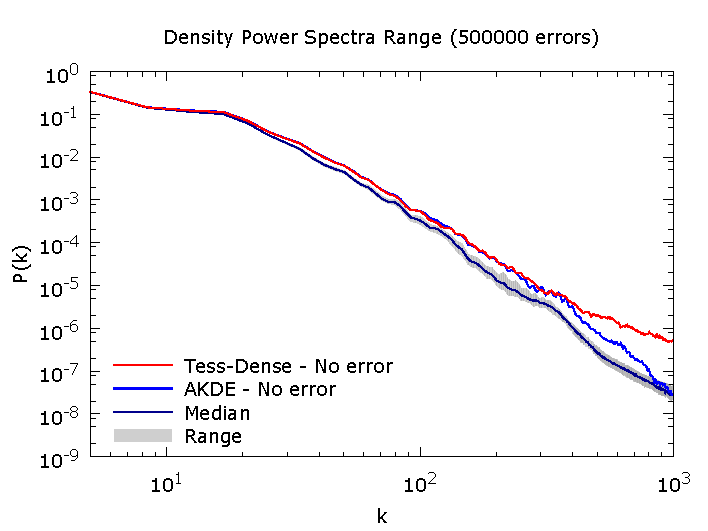
\includegraphics[width=0.32\textwidth]
		{\rootPath Figures/hacc/psd-errors/trace_255_akde_err500000.pdf}
	\caption{Bitflip influence on AKDE power spectrum range}
	\label{fig:hacc:corrupted:spectrum}
\end{figure*}








Using the power spectrum comparaison metrics (see equation~\ref{eq:psd_metric})
we can see the variation of the distance between analytical and corrupted
results as a function of the corruption rate. Those results are visible in
figure~\ref{fig:synthetic:corrupted:powerspectrum-integral}. This figure also
shows, for information, an horizontal line showing the distance between
Tess-Dense and AKDE mean results. This line therefore represent the threshold of
variability between methods. Curve points bellow this threshold represent input
set for which the effect of data corruption is smaller than the difference we
can expect between different methods.

\begin{figure*}[p]
	\centering
	\includegraphics[width=0.9\textwidth, page=1]
		{\rootPath Figures/synthetic/pk-integral.pdf}
	\includegraphics[width=0.4\textwidth, page=2]
		{\rootPath Figures/synthetic/pk-integral.pdf}
	\includegraphics[width=0.4\textwidth]
		{\rootPath Figures/hacc/pk-integral.pdf}
	\caption{Memory corruption influence on synthetic (left) and Hacc (right)
		density field similary (power spectrum integral metric)}
	\label{fig:synthetic:corrupted:powerspectrum-integral}
\end{figure*}




That shows use that corruption could only be detected using redondent
computation with a different method if about $2.5\times10^4$ particles (or more)
are affected, as we this distance has to be twice the inter-method threshold to
be clearly noticeable. Compared to our $1.92\times10^7$ bits input data size,
this gives us a detectable corruption rate thresold of about $0.13\%$














\begin{figure*}[p]
	\centering
	\includegraphics[width=0.4\textwidth]
		{\rootPath Figures/synthetic/Stat-divergence.pdf}
	\includegraphics[width=0.4\textwidth]
		{\rootPath Figures/hacc/Stat-divergence.pdf}
	\caption{Memory corruption influence on synthetic (left) and Hacc (right)
		density field similary (statistical metrics)}
	\label{fig:synthetic:corrupted:statistical-distance}
\end{figure*}

\begin{figure*}[p]
	\centering
	\includegraphics[width=0.9\textwidth, page=1]
		{\rootPath Figures/synthetic/kolmogorov-integral.pdf}
	\includegraphics[width=0.4\textwidth, page=2]
		{\rootPath Figures/synthetic/kolmogorov-integral.pdf}
	\includegraphics[width=0.4\textwidth]
		{\rootPath Figures/hacc/kolmogorov-integral.pdf}
	\caption{Memory corruption influence on synthetic (left) and Hacc (right) 
		density field similary (kolmogorov integral metric)}
	\label{fig:synthetic:corrupted:kolmogorov-distance}
\end{figure*}







%=====================================================================
%=====================================================================
\ifstandalone
	\bibliographystyle{apalike}
	\bibliography{\rootPath Annexes/biblio}
\fi
%=====================================================================
%=====================================================================
\end{document}
